\documentclass[]{article}

\usepackage{amsfonts}
\usepackage{amsmath}
\usepackage{graphicx}
\usepackage{amsthm}
\usepackage{svg}
\usepackage{enumitem}
\usepackage{color}
\usepackage{float}


\graphicspath{{images/}}
\setsvg{svgpath={./images/}}

\newtheorem{thm}{Theorem}[section]
\newtheorem{Def}{Definition}[section]
\newtheorem*{thm*}{Theorem}
\newtheorem*{def*}{Definition}
\newtheorem{lem}{Lemma}[section]
\newtheorem*{rem}{Remark}
\newtheorem*{conj}{Conjecture}

\newcommand{\compav}[1]{\textbf{\textcolor{blue}{#1}}}
\newcommand{\compat}[1]{\textbf{\textcolor{red}{#1}}}
\newcommand{\shiftleft}[2]{\makebox[0pt][r]{\makebox[#1][l]{#2}}}
\newcommand{\tilda}{\big{\char"7E}}



%opening
\title{Recurrence of Geodesic Flow on the Necker Cube Surface}
\date{}
\author{Pavel Javornik}

\begin{document}


\maketitle



\begin{center}

\includesvg[width=4.8in]{cubecoverphoto}\\
\end{center}

\begin{abstract}
\compav{Still working on the abstract}
This paper classifies the periodic and drift-periodic rational trajectories on the Necker cube surface, a periodic surface built out of squares popular in optical illusions. By studying the branched cover of the Necker cube with translational and rotational symmetries, we can deduce from the structure of its quotient exactly which conditions of the initial trajectory angles are necessary to close on the Necker surface. The $\mathbb Z^2$-cover of the quotient is a branched cover of the Necker cube. As such, any closed paths lifted onto the cover will close on the surface as well. An affine automorphism of the quotient extends to an isomorphism of its absolute Homology, which is dual to its derivative, an element of the surface's Veech group, acting on a paths rational direction identified with $\mathbb{Z}^2$. 
\end{abstract}



\newpage
\section{Introduction}

\compav{Started here on Aug. 3 (I've made changes all the way until my next blue comment. )}

The Necker cube[citation] has made numerous appearances throughout history. The artist famous for his use of optical illusions in his work, M.C. Escher, has occasionally used tilings of the Necker cube such as in the lithographs ``Metamorphosis I," and ``Convex and Concave." (Pictured below.) The crystallographer Louis Albert Necker was credited for having extensively studied the Necker cube's geometry[citation] and remarked on this simple, yet fascinating, optical illusion that appears to ``simultaneously protrude from and intrude into the page."[citation:wolfram] Those who feel nostalgic might have even realized it is the same board in which ``Q*bert" hops around on in the 1982 arcade game. [cite?]

\begin{figure}[H]
\begin{center}
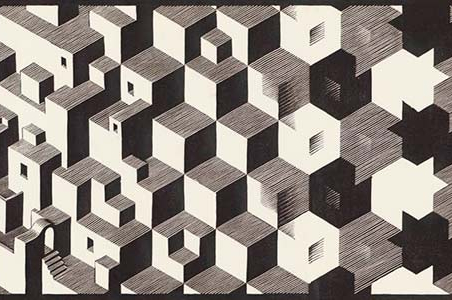
\includegraphics[scale=0.4]{escher.jpg}
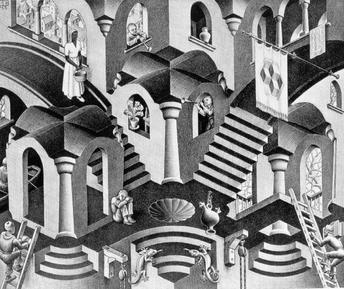
\includegraphics[scale=0.55]{escher2.jpg}
\caption{The Necker cube tiling as it appears briefly in ``Metamorphosis I," and hung on a banner in ``Convex and Concave."[citation]}
\label{fig:Escher}
\end{center}
\end{figure}

The tiling of the Necker cube is what we mean when we refer to the Necker cube surface, denoted $\mathbf S$. There are $\mathbb R^3$ translational symmetries of its embedded form in space that allows it to be tiled periodically. Studying such a surface naturally begs the question of whether or not straight-line paths traveling on the surface are ever periodic. And if so, is there a way to classify all such paths? Could there even be some intrinsic property 
\begin{figure}[H]
\centering
\includesvg[width=1.5in]{cubesxyzpaths2}
\caption{Some periodic and drift-periodic trajectories show us that the inital direction of a geodesic most likely determines its periodicity.}
\end{figure}


In fact there is a remarkably simple solution to this problem. Let's begin by defining the following subsets of $\mathbb{Z}^2$:

\begin{def*}
Let $v$ be a vector of the form $(x,y)\in\mathbb{Z}^{2}$. We call $v$ an \textbf{odd-odd} vector if x and y are relatively prime and both odd. We denote the \textbf{set of all odd-odd vectors} by $\mathcal{O}$. We say that $v$ is an  \textbf{even-odd} vector if x and y are relatively prime, and x is even if and only if y is odd. We denote the \textbf{set of all even-odd vectors} by $\mathcal{E}$.
\end{def*}

By a fixing a point on the surface $\mathbf S$ and taking a sufficiently small segment of a geodesic (such that it and the point lie on exactly one face of a cube), we construct classes of directions according to the vector direction that the segment travels. The direction is obtained by projecting the segment onto a plane parallel to the face it lies on.

\begin{figure}[H]
\centering
\includesvg{vectorplane}
\end{figure}

The set of equivalence classes of directions on $\mathbf S$ is $\mathbb R/\frac{\pi}{2}\mathbb Z$ (a consequence of $\mathbf S$'s rotational symmetries), whose rational angles are then identified with the sets $\mathcal{O}$ and $\mathcal{E}$. Now if the geodesic has an initial direction identified with an element of $\mathcal{O}$, it is periodic on $\mathbf S$. But if that direction is identified with an element of $\mathcal{E}$, then the geodesic is drift-periodic. Otherwise, the geodesic has an irrational initial trajectory and is [yet to be decided] on $\mathbf S$. More formally stated, we have the following theorem:

\begin{thm*}
Yet to be written
\end{thm*}

\subsection{Some Background}
This paper assumes that the reader is familiar with fundamental concepts in algebraic topology, such as covering space theory and the study of Veech surfaces and associated Veech groups. In order to prove this theorem, we take a number of covers of a surface isometric to $\mathbf S$. Our goal then is to take a branched cover of the surface as four "copies" of that surface, and rotate these copies so as to align the geodesic flow and identify edges solely by translation. The quotient space obtained by modding out this surface by its translational symmetries is translation and Veech.

The Veech surface has an $SL(2,\mathbb{R})$-commensurable Veech group characterized as derivatives of affine maps of the translation surface. Such affine diffeomorphisms of the surface induce isomorphisms of its absolute homology (with coefficients in $\mathbb Q$). We obtain the direction of a closed geodesic flow from its holonomy vector and show that the odd-odd directions closing on the translation cover, and consequently $\mathbf S$, remains invariant given that the flow of a geodesic with slope one closes on the cover. This translation cover is considered a $\mathbb{Z}^2$-cover of the veech surface. We associate its fundamental group with the kernel of a homomorphism from the closed paths of its Veech surface quotient to $\mathbb{Z}^2$. There are numerous dualizations to be made between homologies, homology classes, and $SL(2,\mathbb{R})$ action on $\mathbb{Z}^2$ in order to solve this problem.

\begin{rem}
The initial approach of taking four ``copies" of the surface as a branched cover of $\mathbf S$ was in many ways inspired by the method in which [such and such]'s work on the dynamics of geodesic flow on the Ehrenfest-Wind Tree Model.[citation]. In fact the Wind Tree and the Necker cube surface have much in common in terms of which initial trajectory angles determine periodicity. The two differ, however, in regards to whether or not the initial point of the flow has an effect on periodicity. Although the translation surfaces obtained are near identical, the manners in which they are obtain differ greatly. A billiard flow is realigned by a series of reflections of the original surface by stringing copies of polygons along a ``laundry line" until a translation surface is obtained. On the other hand, $\mathbf S$ exhibits rotational symmetries that we exploit to obtain our translation surface.
\end{rem}
\subsection{Acknowledgements}
to do: 

- Hooper

- Artigiani "Exceptional Ergodic Directions" for Notation

- Vincent, Ferran and Pascal if I can get a rough draft of their book

- Hubert, et. al. "Recurrence flow " paper on wind tree

- Ariel Mazur for assistance earlier on

- Math dept at CCNY? or research internship? Not sure if apropos.

\section{Constructing and Flattening $\mathbf{S}$}

This section will detail how the Necker cube surfaces is constructed as the union of infinitely many Necker cubes. Each Necker cube is taken to be the union of unit squares, each belonging to one of three orthogonal auxiliary planes. An isometric variant of $\mathbf{S}$ can be described as a \emph{flattening} of $\mathbf{S}$ such that these unit squares all lie on the $x$-$y$ plane.

\begin{figure}[H]
\begin{center}
\includesvg[width=2in]{cubesxyz}
\caption{The Necker cube surface embedded in space.}
\label{fig:cubexyz}
\end{center}
\end{figure}

\subsection{The Necker Cube Surface}

The set $\mathbf{S}$ is built periodically out of infinitely many Necker cubes (a union of three unit squares). To each square fix a label, A,B, or C. For every integer triple, $(m,n,p)$, in $\mathbb R^3$, we have the following:

\vspace{0.2in}
\begin{tabular}{p{10cm}c}
\begin{align*}
\mathbf{A}_{m,n,p} = [m, m+1]\times[n,n+1]\times\{p\}, 
\\\mathbf{B}_{m,n,p} = \{m+1\}\times[n,n+1]\times[p-1,p],
\\\mathbf{C}_{m,n,p}= [m,m+1]\times\{n+1\}\times[p-1,p].
\end{align*}
&
\shiftleft{0.8in}{\raisebox{-1in}{
\includegraphics[scale=1]{label.png}}}
\end{tabular}

The Necker cube surface is obtained as the union of infinitely many Necker cubes that satisfy the condition that $m+n+p=0$. $\mathbf{S}$ can be separated into the following sets:

\begin{align*}
\mathbf{A}=\bigcup\big{\{}\mathbf{A}_{m,n,p}: m+n+p=0\big{\}},
\\\mathbf{B}=\bigcup\big{\{}\mathbf{B}_{m,n,p}: m+n+p=0\big{\}},
\\\mathbf{C}=\bigcup\big{\{}\mathbf{C}_{m,n,p}: m+n+p=0\big{\}}.
\end{align*}

\noindent We can now give a set definition of the Necker cube surface.

\begin{Def} The \textbf{Necker cube surface}, denoted $\mathbf{S}$, is the surface made up of the union of unit squares of the form $\mathbf{S} = \mathbf{A}\cup\mathbf{B}\cup\mathbf{C}$.\end{Def}

\subsection{The Flattened Form}
The Necker cube surface is path-isometric to a topological quotient of a particular subset of the plane. We call the flattened form $\mathbf{U}$, and the subset of the plane $\mathbf P$ (See figure $\ref{fig:uprimeu}$).
The subset $\mathbf P$ is the region of the plane with unit squares removed:
\begin{equation}
\label{eq:P}
\mathbf{P} = \mathbb{R}^{2}\text{ }\backslash\bigcup_{m,n \in {\mathbb Z}} \big{\{}(u,v):u\in(2m-\frac{1}{2},2m+\frac{1}{2}),\text{ } v\in(2n-\frac{1}{2},2n+\frac{1}{2})\big{\}}.
\end{equation}

\begin{figure}[H]
\begin{center}
\includesvg[width=1.5in]{uprime}
\end{center}
\caption{$\mathbf P$ is real plane with unit squares removed at every even integer pair.}
\label{fig:uprimeu}
\end{figure}

\noindent We define a relation on $\mathbf P$ that identifies the sides of the boundaries of each hole in pairs. Each side is identified with another side of the same hole by rotation about the bottom left or top right corners of the hole by $\pm\frac{\pi}{2}$. The result is the following edge identifications made on cut out square holes: 

\begin{figure}[H]\centering
\includesvg[width=2in.]{quotient}
\end{figure}

\begin{Def}{} $\mathbf U$ is the surface obtained as the topological quotient $\mathbf P/\mathbf R$, where $\mathbf R$ is defined as follows:
\begin{gather*}
\text{Let } x_{0}=(u_{0},v_{0}),x_{1}=(u_{1},v_{1}) \in \mathbf{P}.  \mathbf{ R} \text { is given as the relation } x_{0}\mathbf{R}x_{1} \\ \text{ iff } x_{0}=x_{1}
 \text{ or, for }x_{0},x_{1} \in {\partial} \left( \left[2m-\frac{1}{2},2m+\frac{1}{2}\right] \times \left[2n-\frac{1}{2},2n+\frac{1}{2}\right] \right)\\
 \text{ and }m,n\in\mathbb{Z},
  \left[\begin{array}{c}
u_{1} -2m
\\v_{1}-2n
\end{array}\right] = \left[\begin{matrix}
0 && 1\\
1 && 0
\end{matrix}\right]
\left[ \begin{array}{c}u_{0}-2m\\
v_{0}-2n
\end{array}\right]
. \end{gather*}
\end{Def}

We can see that $\mathbf{U}$ is a Euclidean cone surface with infinitely many singularities of cone angles $\frac{3\pi}{2}$ and $6\pi$. Observe that $\mathbf{S}$ is also a cone surface with as many singularities of the same cone angles.

\subsection{A Path Isometry From $\mathbf S$ to $\mathbf U$}
A path-isometric map from $\mathbf{S}$ to $\mathbf{P}$ induces an isometry from the Necker cube surface to $\mathbf{U}$. The path isometry $\Psi:\mathbf{S}\rightarrow\mathbf{P}$ is a piece-wise, well-defined map that is given as a linear transformation in which a square labeled $\mathbf{A}$, $\mathbf{B}$, or $\mathbf{C}$ is mapped to its corresponding square on $\mathbf{P}$. $\Psi$ is  essentially a transformation that cuts along the edges parallel with the z-axis. (See figure $\ref{fig:cut}$)

\begin{figure}[H]
\includesvg[width=2.1in]{cubesxyzcut}
\raisebox{0.4in}{\includesvg[width=2.3in]{unfoldcut}}
\caption{The images of $\mathbf S$ and $\Psi(\mathbf{S})$ with edges identified.}
\label{fig:cut}
\end{figure}

\begin{Def}
The bijective function $\Psi$ maps all of $\mathbf{S}$ to $\mathbf P$, and is given as:
\end{Def}

\begin{equation}
\Psi\left[\begin{array}{c}
	x\\y\\z
\end{array}\right] 
= 
\begin{cases}
	\left[ \hspace{2mm} \begin{matrix}
		1 & 0 & 0 \\
		0 & 1 & 0 \\
		0 & 0 & 1
	\end{matrix}\hspace{3mm}\right]

	\left[\begin{array}{c}
	x - \left\lfloor x \right\rfloor
	\\ y- \left\lfloor y \right\rfloor
	\\ -(z - \left\lfloor z \right\rfloor)
	\end{array} \right]
	+
	\left[\begin{array}{c}
		2 \left\lfloor x \right\rfloor - 1
		\\ 2\left\lfloor y \right\rfloor - 1
		\\ z - \left\lfloor z \right\rfloor
	\end{array} \right]
		& \text{if } (x,y,z)\in A	\vspace{2mm}
	\\
		
		
	\left[ \begin{matrix}
	0 & 0 & 1 \\
	0 & 1 & 0 \\
	-1 & 0 & 0
	\end{matrix}\hspace{2mm}\right]
	\left[\begin{array}{c}
		x - \left\lfloor x \right\rfloor
		\\ y- \left\lfloor y \right\rfloor
		\\ -(z - \left\lfloor z \right\rfloor)
		\end{array} \right]
	+
		\left[\begin{array}{c}
			2 \left\lfloor x \right\rfloor - 1
			\\ 2\left\lfloor y \right\rfloor - 1
			\\ x - \left\lfloor x \right\rfloor
		\end{array} \right]
			& \text{if } (x,y,z)\in B	\vspace{2mm}
	\\
	
		\left[ \begin{matrix}
		1 & 0 & 0 \\
		0 & 0 & 1 \\
		0 & -1 & 0
		\end{matrix}\hspace{2mm}\right]
		\left[\begin{array}{c}
			x - \left\lfloor x \right\rfloor
			\\ y- \left\lfloor y \right\rfloor
			\\ -(z - \left\lfloor z \right\rfloor)
			\end{array} \right]
		+
			\left[\begin{array}{c}
				2 \left\lfloor x \right\rfloor - 1
				\\ 2\left\lfloor y \right\rfloor - 1
				\\ y - \left\lfloor y \right\rfloor
			\end{array} \right]
				& \text{if } (x,y,z)\in C	\vspace{2mm}
\end{cases}
\end{equation}

Clearly, $\Psi$ preserves distances on the faces of each as it consists entirely of rotations and translations. As such, it is path-isometric and induces an isometry between the Necker Cube surface and $\mathbf U$.

\begin{thm}{$\mathbf{S}$ is isometric to  $\mathbf{U}$.}
\begin{proof}

Let $(\mathbf{S}, d)$ and $(\mathbf{U}, d')$ be metric spaces with their respective metrics. Let $a,b\in\mathbf{S}$, and suppose that $\Psi(a)=a',\Psi(b)=b'\in\mathbf{U}$. We will denote the distance between $a$ and $b$ by $D=d(a,b)$, and the distance between $a'$ and $b'$ by $D'=d'(a',b')$. Since $\Psi$ and $\Psi^{-1}$ are linear transformations that act on subsets of auxiliary planes in $\mathbb{R}^{3}$, the images of any curves on $\mathbf{S}$ or $\mathbf{U}$ under these maps will not be deformed and retain their lengths. Thus $D \leq d'(\Psi(a), \Psi(b)) = d'(a',b') = D'$. Likewise $D' \leq d(\Psi^{-1}(a'),\Psi^{-1}(b')) = d(a,b) = D$. Therefore $D=D'$, and $\Psi$ and $\Psi^{-1}$ preserves distances between points. And so, $\mathbf{S}\simeq\mathbf{U}$.
\end{proof} 
\end{thm}

\newpage
%\subsection{Flattening $\mathbf{S}$}
%This section will describe the isomorphic map $\Psi:\mathbf{C}\rightarrow\mathbf{U}$, its inverse, $\Psi^{-1}:\mathbf{U}\rightarrow\mathbf{C}$, and prove that $\mathbf{C}$ and $\mathbf{U}$ are isometric.
%
%The flattening procedure can be represented as a series of cuts made along edges parallel to the z-axis. The gluing structure is preserved by the relations defined on $\textbf{U}$ and $\textbf{U}'$. 
%
%
%$\Psi$ is defined piecewise, and denote each subset of $\mathbf{C}$ with the letters $A$, $B$, $C$. We do the same for $\mathbf{U}$ but use instead $A'$, $B'$, $C'$. 
%
%\begin{gather*}
%	\text{Let }x,y,z\in\mathbb{R}. \text{ Then}
%	\\A=\bigcup\big\{\mathbf{C}\cap\{(x,y,p)\in\mathbb{R}\}: p\in\mathbb{Z}\big\}
%	\\B=\bigcup\big\{\mathbf{C}\cap\{(x,n,z)\in\mathbb{R}\}: n\in\mathbb{Z}\big\}
%	\\C=\bigcup\big\{\mathbf{C}\cap\{(m,y,z)\in\mathbb{R}\}: m\in\mathbb{Z}\big\}
%	\\\text{are the collection of the faces of cubes that lie on planes that are parallel to one another.}
%	\\\text{As shown here:}
%\end{gather*}
%
%
%
%To describe the subsets $A'$, $B'$, and $C'$ properly we will introduce the function $\mu_{n}:\mathbb{R}\rightarrow \left[0,n\right) $ as shorthand for the family of functions that take a real number to its residue class of reals modulo n, for some integer n.
%
%\begin{gather*}
%	\text{Let }u,v\in\mathbb{R}. \text{Then }
%	\\A'= \{(u,v,0): 0<\mu_{2}(u)\leq 1 ,\hspace{4mm} 0<\mu_{2}(v)\leq 1\}
%	\\B'= \{(u,v,0): 1<\mu_{2}(u)\leq 2,\hspace{4mm} 0<\mu_{2}(v)\leq 1\}
%	\\C'= \{(u,v,0): 0<\mu_{2}(u)\leq 1,\hspace{4mm} 1<\mu_{2}(v)\leq 2\}
%	\\\text{are the collections of the associated faces of the flattened structure.}
%\end{gather*}
%
%
%
%Now we will define $\Psi$ piecewise.
%
%
%
%We chose to preserve the matrix structure in order to emphasize the manner in which every square is taken to $\mathbf{U}$ from $\mathbf{C}$ and vice-versa. The negations of some of these variables are a result of this structure being built so as the integer triples lie on the plane $z=-(x+y)$. Defining the maps this way also makes it possible to generalize it for any surface constructed in a similar manner of taking unions of three faces of rectangular prisms in real space. (i.e. $\chi_{m,n,p}$ belongs to a larger family of rectangular arrangements parameterized by the dimensions of the rectangular prism. In this case, $\chi_{m,n,p}$ is a member of this family whose dimensions are $1\times1\times1$). 
%
%Now we will define the inverse map, $\Psi^{-1}$, in a similar manner. 
%
%\begin{equation}
%	\Psi^{-1}\left[\begin{array}{c}
%		x\\y\\z
%	\end{array}\right] 
%	= 
%	\begin{cases}
%		\left[ \hspace{2mm} \begin{matrix}
%			1 & 0 & 0 \\
%			0 & 1 & 0 \\
%			0 & 0 & 1
%		\end{matrix}\hspace{3mm}\right]
%	
%		\left[\begin{array}{c}
%		x - 2\left\lfloor \frac{x}{2} \right\rfloor
%		\\ y- 2\left\lfloor \frac{y}{2} \right\rfloor
%		\\ z
%		\end{array} \right]
%		+
%		\left[\begin{array}{c}
%			\left\lfloor \frac{x}{2} \right\rfloor
%			\\ \left\lfloor \frac{y}{2} \right\rfloor
%			\\ -(\left\lfloor \frac{x}{2} \right\rfloor + \left\lfloor \frac{y}{2} \right\rfloor )
%		\end{array} \right]
%			& \text{if } (x,y,z)\in A'	\vspace{2mm}
%		\\
%		\left[ \hspace{2mm} \begin{matrix}
%			0 & 0 & -1 \\
%			0 & 1 & 0 \\
%			1 & 0 & 0
%		\end{matrix}\hspace{0mm}\right]
%	
%		\left[\begin{array}{c}
%		-(x - 2\left\lfloor \frac{x}{2} \right\rfloor)
%		\\ y- 2\left\lfloor \frac{y}{2} \right\rfloor
%		\\ z
%		\end{array} \right]
%		+
%		\left[\begin{array}{c}
%			1+\left\lfloor \frac{x}{2} \right\rfloor
%			\\ \left\lfloor \frac{y}{2} \right\rfloor
%			\\ -(\left\lfloor \frac{x}{2} \right\rfloor + \left\lfloor \frac{y}{2} \right\rfloor -1)
%		\end{array} \right]
%			& \text{if } (x,y,z)\in B'	\vspace{2mm}
%
%	\\
%	
%		\left[ \hspace{2mm} \begin{matrix}
%			1 & 0 & 0 \\
%			0 & 0 & -1 \\
%			0 & 1 & 0
%		\end{matrix}\hspace{0mm}\right]
%	
%		\left[\begin{array}{c}
%		x - 2\left\lfloor \frac{x}{2} \right\rfloor
%		\\ -(y- 2\left\lfloor \frac{y}{2} \right\rfloor)
%		\\ z
%		\end{array} \right]
%		+
%		\left[\begin{array}{c}
%			\left\lfloor \frac{x}{2} \right\rfloor
%			\\1+ \left\lfloor \frac{y}{2} \right\rfloor
%			\\ -(\left\lfloor \frac{x}{2} \right\rfloor + \left\lfloor \frac{y}{2} \right\rfloor -1)
%		\end{array} \right]
%			& \text{if } (x,y,z)\in B'	\vspace{2mm}
%			
%	\end{cases}
%\end{equation}
\section{The Four-Fold Cover and Translation Surface}
\compat{Revisit to make sure it summarizes the section}


\subsection{Four-Fold Cover of $\mathbf{U}$}
A geodesic on $\mathbf{U}$ viewed as a sequence of line segments on $\mathbf{P}$ travels in at most four directions which differ by a rotation of a multiple of $\frac{\pi}{2}$. This is a consequence of the edge identifications taking the boundary of a hole on $\mathbf{P}$ to its counterpart by a rotation of ninety degrees. To each of these directions we associate an element of $\mathbb{Z}/4\mathbb{Z}$ to signify one of the four possible directions of the geodesic flow at any given time. Given that, we can create a four-fold cover of $\mathbf{U}$ as a topological quotient of $\mathbf{P}\times\mathbb{Z}/4\mathbb{Z}$. For every integer pair centered around every hole of $\mathbf{P}\times\mathbb{Z}/4\mathbb{Z}$, create the edge identifications that takes one plane to the next in the following manner:

\begin{figure}[H]
\centering
\includesvg[width=4in]{utilda}
\label{fig:utilda0}
\caption{$\tilde{\mathbf{U}}_0$ is a branched cover of $\mathbf{U}$ of degree four.}
\end{figure}

$\tilde{\mathbf{U}}_0$ has the obvious covering map that takes every point on $\tilde{\mathbf{U}}_0$ and projects it onto $\mathbf{U}$. We define the edge identifications as a relation on $\mathbf{P}\times\mathbb{Z}/4\mathbb{Z}$. For $i\in[-\frac{1}{2},\frac{1}{2}]$:



\begin{equation}
\begin{split}
(2m+i, 2n-\frac{1}{2};j)\sim(2m-\frac{1}{2},2n+i;j+1)\\
(2m+i, 2n+\frac{1}{2};j)\sim(2m+\frac{1}{2},2n+i;j+1)\\
\vspace{0.2in}\text{for } (m,n;j) \in \mathbb{Z}^{2}\times\mathbb{Z}/4\mathbb{Z}.
\label{eq:rel2}
\end{split}
\end{equation}

We define $\tilde{\mathbf{U}}_0$ to be the topological quotient, $(\mathbf{P}\times\mathbb{Z}/4\mathbb{Z})/\sim$. $\tilde{\mathbf{U}}_0$ is a Euclidean cone surface with four vertices at each hole centered at $(2m,2n;\mathbb{Z}/4\mathbb{Z})$ of cone angle $6\pi$.

\subsection{Symmetries of $\tilde{\mathbf{U}}_0$}
There are certain translational and rotational symmetries of $\mathbf{P}\times\mathbb{Z}/4\mathbb{Z}$ that we use to define isometries. These isometries are well-defined and induce isometries on $\tilde{\mathbf{U}}_0$ that respect the edge identifications we made earlier.

\begin{Def}Let $m,n\in\mathbb{Z}$. The {family of translation maps}, $\mathbf{T}^{m,n}_{0}$ on $\mathbf{P}\times\mathbb{Z}/4\mathbb{Z}$, is given as $\mathbf{T}^{m,n}_{0}(u,v;j)=(u+2m,v+2n;j)$.\newline
The {family of ``rotational" isometries} on $\mathbf{P}\times\mathbb{Z}/4\mathbb{Z}$ is given as the automorphism $\mathbf{R}_0(u,v;j)=(u,v;j+1)$, where $\mathbf{R}_0$ is an action on $\mathbf{P}\times\mathbb{Z}/4\mathbb{Z}$ of order 4.
\end{Def}

\begin{lem}$\mathbf{T}^{m,n}_{0}$ induces a well-defined isometry on $\tilde{\mathbf{U}}_0$.
\begin{proof}
It suffices to show that $\mathbf{T}^{m,n}_{0}$ preserves the edge identifications $\eqref{eq:rel2}$. Let $x,y\in\mathbf{P}\times\mathbb{Z}/4\mathbb{Z}$, where $x=(u_x,v_x;j_x)$ and $y=(u_y,v_y,j_y)$. Clearly, if $x=y$, then $\mathbf{T}^{m,n}_{0}(x)=\mathbf{T}^{m,n}_{0}(y)$. Hence, $T_0$ is bijective. Consider the case where $x\neq y$. Let $x\sim y$ and observe that if $x,y$ lie on any of the edges, then $\mathbf{T}^{m,n}_{0}(x)=(u_x+2m,v_x+2n;j_x)$ and $\mathbf{T}^{m,n}_{0}(y)=(u_y+2m,v_y+2n;j_y)$ for $m,n\in\mathbb{Z}$. Since $x\sim y$, either $j_y=j_x+1$, or $j_x=j_y+1$. Suppose the former is true. Then for $i$ in the interval $[-\frac{1}{2},\frac{1}{2}]$:

\begin{equation*}
\begin{split}
(2m_x+2m+i, 2n_x+2n-\frac{1}{2};j_x)\sim(2m_x+2m-\frac{1}{2},2n_x+2n+i;j_y)\\\text{ and }\hspace{2in}\\
(2m_x+2m+i, 2n_x+2n+\frac{1}{2};j_x)\sim(2m_x+2m+\frac{1}{2},2n_x+2n+i;j_y),\\
\end{split}
\end{equation*}
which is the result of $T_0$ acting on the edges, and $m_x,n_x$ are integers that originally ensured that $x\sim y$. Since $m,n$ are arbitrarily chosen integers, $T_0$ maps one edge to exactly one other as the edges surrounding each hole are indexed by a unique pair of even integers and $T_0$  is a bijective map that respects that construction. A similar argument holds for the case where $j_x=j_y+1$. Therefore, $\mathbf{T}^{m,n}_{0}(x)\sim\mathbf{T}^{m,n}_{0}(y)$.
\end{proof}
\end{lem}

We will call the induced isometry on $\tilde{\mathbf{U}}_0$, $\bar{\mathbf{T}}^{m,n}$.

\subsection{Four-fold Translation Cover}

 Now we will show that $\tilde{\mathbf{U}}_0$ is isometric to a translation surface via another induced isometry on $\mathbf{P}\times\mathbb{Z}/4\mathbb{Z}$. We would like this map to rotate each individual plane of $\mathbf{P}\times\mathbb{Z}/4\mathbb{Z}$ about the origin in such a way that edges one the boundaries are identified strictly by translation. Every plane that is represented as an element of $\mathbb{Z}/4\mathbb{Z}$ is conveniently acted on by a ninety degree rotation matrix, whose power we take to be that very same element.


We express $\phi:\mathbf{P}\times\mathbb{Z}/4\mathbb{Z} \rightarrow \mathbf{P}\times\mathbb{Z}/4\mathbb{Z}$ as $\phi(u,v;j) = (u',v';j)$, where

\begin{equation}
	\left[\begin{array}{c}
		u'\\v'
	\end{array}\right] =
		\left[ \hspace{1mm} \begin{matrix}
				0 & 1\\
				-1 & 0
			\end{matrix}\hspace{1mm}\right]^{j}\left[\begin{array}{c}
					u\\v
				\end{array}\right].
\label{eq:phi}
\end{equation}
This is clearly an isometry, as rotations preserve distance and $j\mapsto j$.

\begin{Def} Let $\sim$ be the equivalence relation $\eqref{eq:rel2}$, and $\phi$ be the isometric map on $\mathbf{P}\times\mathbb{Z}/4\mathbb{Z}$ $\eqref{eq:phi}$. Define a new relation obtained from $\sim$ as $x_1\sim_{\phi}x_2$ iff $\phi^{-1}(x_1) \sim \phi^{-1}(x_2)$ for $x_1,x_2\in\mathbf{P}\times\mathbb{Z}/4\mathbb{Z}$. A new surface is obtained as the topological quotient $\tilde{\mathbf{U}}=$ $(\mathbf{P}\times\mathbb{Z}/4\mathbb{Z})/\sim_{\phi}$.\label{eq:simphi}
\end{Def}


\begin{figure}[H]
\centering
\includesvg[width=3.65in]{utildaprime}
\caption{$\tilde{\mathbf{U}}$ with edges identified, and holes indexed relative to $\mathbf{P}\times\{0\mod{4}\}$.}
\label{fig:utilda}
\end{figure}


\begin{thm}{The following statements are true:}
\begin{enumerate}[label=(\roman*)]
\item The map $\phi$ induces a well-defined isometry from $\tilde{\mathbf{U}}_0$ to $\tilde{\mathbf{U}}$.
\item $\tilde{\mathbf{U}}$ is a translation surface.
\end{enumerate}
\begin{proof}
It will again suffice to show that $\phi$ preserves $\tilde{\mathbf{U}}_0$'s edge identifications to prove $(i)$. Let $x_1,x_2\in\mathbf{P}\times\mathbb{Z}/4\mathbb{Z}$. From $\tilde{\mathbf{U}}$'s definition $\eqref{eq:simphi}$, we see that $x_1\sim_{\phi} x_2$ if and only if $\phi^{-1}(x_1) \sim \phi^{-1}(x_2)$. By taking $\phi^{-1}(x_1)$ and $ \phi^{-1}(x_2)$ to be the pre-images of the quotient map onto $\tilde{\mathbf{U}}_0$, it is clear that $\phi$ preserves identifications. Otherwise, it would contradict the definition. Furthermore, since $\phi$ is a well-defined isometry, there is an induced isometry on the topological quotients, $\tilde{\mathbf{U}}_0$ and $\tilde{\mathbf{U}}$.\newline
Let $x_1\sim_{\phi} x_2$. Then $\phi^{-1}(x_1) \sim \phi^{-1}(x_2)$. Let $\phi^{-1}(x_1)=(u_1,v_1;j_1)$ and $\phi^{-1}(x_2)=(u_2,v_2;j_2)$. Without loss of generality, suppose that $j_2=j_1+1$. Let $i$ vary over the interval $[-\frac{1}{2},\frac{1}{2}]$, and $m,n$ be integers such that they satisfy the relation $\phi^{-1}(x_1) \sim \phi^{-1}(x_2)$. If $\phi$ acts on these these two points, then $x_1 = (u_1',v_1';j_1)$ and $x_2 = (u_2',v_2';j_1+1)$. But we know that $(u_1',v_1')=M^{j_1}(u_1,v_1)$ and $M^{j_1+1}(u_2',v_2')=(u_2,v_2)$, where $M$ is the rotation matrix as in $\phi$. Thus, $M^{j_1}(u_1,v_1)\times\{j_1\}\sim_\phi M^{j_1+1}(u_2,v_2)\times\{j_1+1\}$. By multiplying through by $M^{-j_1}$ prior to taking the cross-product, we obtain $(u_1,v_1)\times\{j_1\}\sim_\phi M(u_2,v_2)\times\{j_1+1\}$. Since $M(u_2,v_2) = (v_2,-u_2)$, we can express the relation $\sim_\phi$ as
\begin{equation*}
\begin{split}
(2m+i, 2n-\frac{1}{2};j_1)\sim_\phi(2n+i, -(2m-\frac{1}{2});j_1+1),\\
\text{ and }\hspace{1.2in}\\
(2m+i, 2n+\frac{1}{2};j_1)\sim_\phi(2n+i, -(2m+\frac{1}{2});j_1+1).\\
\end{split}
\end{equation*}
It is clear from this relation and figure $\ref{fig:utilda}$ that $\tilde{\mathbf{U}}$ is a translation surface.
\end{proof}
\end{thm}
We will denote this induced isometry as $\bar{\phi}$.

%A geodesic on this translation surface can be realized as a sequence of edge crossings on the phase planes. By taking a quotient of this surface, a closed straight-line path can be lifted from the quotient onto $\tilde{\mathbf{U}}$, and then projected onto $\mathbf{U}$ to study geodesic behavior of any given direction.

\subsection{Constructing $\tilde{\mathbf{U}}$'s base surface}
In this section we use the induced isometries on $\tilde{\mathbf{U}}_0$, and the map $\bar{\phi}:\tilde{\mathbf{U}}_0\rightarrow\tilde{\mathbf{U}}$ to define a set of rotational and translational symmetries of $\tilde{\mathbf{U}}$ such that its quotient over the action of these maps are faithful representations of $\tilde{\mathbf{U}}_0$ in terms of how the holes in $\mathbf{P}\times\mathbb{Z}/4\mathbb{Z}$ are indexed. It is briefly mention after the definition of $\tilde{\mathbf{U}}$ that $\bar{\phi}$ alters this scheme relative to $\tilde{\mathbf{U}}_0$. 

\begin{Def}We call the {family of $\tilde{\mathbf{U}}$'s translational symmetries} $\mathbf{T}^{m,n}$ and define it to be the composition of the induced isometric maps: $\mathbf{T}^{m,n}$ = $\bar{\phi}\circ\bar{\mathbf{T}}^{m,n}\circ\bar{\phi}^{-1}$.
\end{Def}

We can see that $\mathbf{T}^{m,n}$ is indeed an isometry on $\tilde{\mathbf{U}}$ as it is composed of the induced isometries, $\bar{\phi}$ and $\bar{\mathbf{T}}^{m,n}$ . We can take the quotient of the translation surface $\tilde{\mathbf{U}}$ over the action of $\mathbf{T}^{m,n}$ to obtain a base surface that realizes $\tilde{\mathbf{U}}$ as an infinite $\mathbb{Z}^2$ cover, where $m,n$ is identified with an integer pair.

\begin{Def}
The translation surface $\mathbf{M}$ is given as a quotient of $\tilde{\mathbf{U}}$ equipped with a  holomorphic 1-form, $(\tilde{\mathbf{U}}/\mathbf{T}^{m,n},\omega)$.
\end{Def} 

\begin{figure}[H]
\centering
\includesvg[width=4in]{mtilda}
\caption{The surface $\mathbf{M}$ with labeled vertices and identified edges. Labels I, II, III, and IV identify the individual planes indexed by \{0,1,2,3\}, respectively.}
\label{fig:mtilda}
\end{figure}

The new surface, $\mathbf M$, is a genus 5 translation surface with the surjective quotient map $f:\tilde{\mathbf{U}}\rightarrow\mathbf M$ that sends every point of $\tilde{\mathbf{U}}$ to its modular equivalent. $\mathbf M$ is a Euclidean cone surface with four singularites of cone angle $6\pi$ on the corners of the square cut out from each of the squares labeled I,II,III, and IV. Those squares have their opposite edges identified by translation. $\mathbf M$ might be thought of as a collection of four $2\times2$ square tori with a unit square cut out from their centers, and identifications made on these edges so as to associate one torus with exactly two others. Although a single edge only relates two of the tori, the vertices in the centers are the same throughout $\mathbf M$.
\newpage

\subsection{$\mathbf M$ as a Veech Surface}
By a series of cutting and gluing operations, $\mathbf M$ has this symmetric representation as a square-tiled staircase (figure $\ref{fig:staircase}$). This is a compact surface with an infinite $\mathbb Z$-cover as the Infinite Staircase. [cite] It shares many of the same symmetries, as well. The vertices of cone angle $2\pi$ can be found on the centers of the squares in the figure below where the black lines intersect. 
\begin{figure}[H]
\centering
\includesvg[width=4in]{mtildastaircase}
\caption{$\mathbf{M}$ as a square-tiled staircase with cone singularities identified.}
\label{fig:staircase}
\end{figure}
As a result of Gutkin-Judge [citation], $\mathbf M$ is a Veech surface whose Veech group is commensurable to $SL(2,\mathbb Z)$. In order to determine which elements of orientation preserving affine diffeomorphisms, denoted Aff$^{+}(\mathbf M)$, have derivatives that belong to the Veech group, V($\mathbf M$), it is necessary to study $\mathbf M$'s various symmetries, as well as its cylinder decomposition.
\vspace{0.1in}

\noindent\textbf{Rotational Symmetries}

One group contained in $V(\mathbf M)$ is SO$(2,\mathbb{Z})$, the group generated by rotations of the square. We want the corresponding affine map of these rotation matrices to obey the convention that we \emph{fix} the second square on the bottom with label I. These maps are unique only up to a translation of the surface and assigning this convention makes it easier to keep track of where the edges of $\mathbf M$ end up. The 90 degree counter-clockwise rotation fixed about the point in the center of that square is denoted $\mathbf{R}$. Its derivative, $\mathbf{R}'$, is the matrix $\left[ \hspace{1mm} \begin{matrix}
							0 & -1\\
							1 & 0
						\end{matrix}\hspace{1mm}\right]$.

\vspace{0.1in}

\noindent\textbf{Translation Symmetries}

The translational symmetries have no unique representation as an element of V($\mathbf M$), as their derivatives are represented as the identity. But they do have an important effect on the surface. Shifting the bottom left-most square to the right and reconstructing the rest by pairing edges is an order 2 homeomorphism denoted $\mathbf{H}$, for horizontal. Likewise, $\mathbf{V}$ is an order 2 homeomorphism that shifts that square upwards. Observe that together they satisfy the property $(\mathbf{H}\mathbf{V})^{6}=(\mathbf{V}\mathbf{H})^{6}=id$. This is essentially moving the squares up the staircase until they come back to where they started, unlike the the group of diagonal translations of the Infinite Staircase that is isomorphic to $\mathbb Z$. The group Trans($\mathbf M$) is isomorphic to the group generated by reflections of a 12-gon, $\mathbb{D}_{12}$.

\vspace{0.1in}

\noindent\textbf{Skew Symmetries}

Observe from the following image that $\mathbf M$ has a uniform cylinder decomposition in both the horizontal and vertical directions:

\begin{figure}[H]
\centering
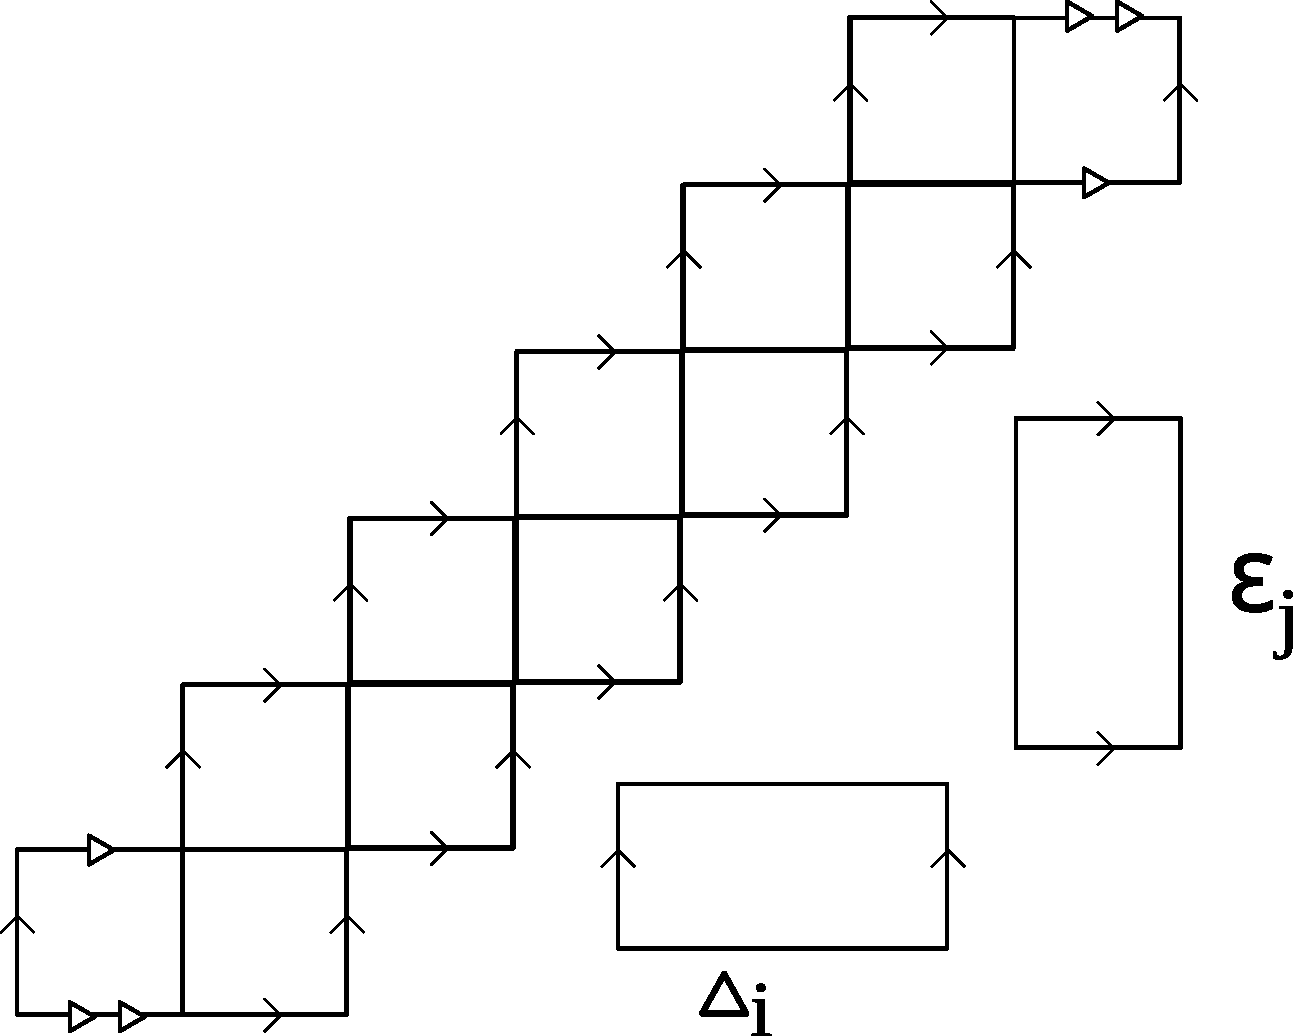
\includegraphics[width=4in]{cylinderdecomp.pdf}
\caption{Horizontal and vertical cylinder decomposition as they overlay and cover the surface.}
\label{fig:decomp}
\end{figure}

Both sets of maximal cylinders are indexed $0\leq i, j \leq 5$. Every cylinder is composed of two unit squares with edges identified by translation. Each cylinder is obtained as a ramified cover of the square torus. We start counting the cylinders from the bottom-most cylinder and increment the index as the cylinders fill the surface going ``up" the staircase. $\small{\mathcal{E}}_0$ is the first cylinder at the bottom whose identifications are \em{not} \normalfont the solid triangles. Travel up the staircase until the laste one, $\small{\mathcal{E}}_5$, the cylinder whose edges are paired by the solid triangles and glue the 12th square with the 1st. $\Delta_{i}$ has the more standard representation starting from the bottom-most horizontal cylinder and going all the way up to the top. 

We define the \emph{inverse modulus} of a cylinder to be the ratio of a cylinders circumference to its width, $\mu^{-1}=\frac{c}{h}$. A \emph{Dehn-twist} of a cylinder is an automorphism of the cylinder of the form  $(x,y)\mapsto(x,y+\mu^{-1} x \mod{h})$, where $x$ and $y$ are points on the cylinder such that x varies along the its circumference. According to [need to cite something], a translation surface whose finite cylinder decompositions in orthogonal directions form a set of inverse moduli. The smallest (rational) common multiple of the set of all these values match up to give a global affine diffeomorphisms of the surface, whose derivatives have the matrix representations
\begin{equation*}
\left[ \hspace{1mm} \begin{matrix}
				1 & \pm \lambda\\
				0 & 1
			\end{matrix}\hspace{1mm}\right] \text{ and }
			\left[ \hspace{1mm} \begin{matrix}
							1 & 0\\
							\pm \lambda & 1
						\end{matrix}\hspace{1mm}\right],
\end{equation*}
such that $\lambda$ is that lowest common multiple. [cite]

Let $\mu^{-1}_{\Delta_i},\mu^{-1}_{\mathcal{E}_j}$ denote the inverse moduli of the cylinders. The cylinders $\Delta_{i}$ and $\small{\mathcal{E}}_j$, as i and j vary, all have the same inverse moduli since they are all defined as two unit squares with identifications made by translation. Therefore, $\lambda=$ l.c.m.($\mu^{-1}_{\Delta_i}\cup\mu^{-1}_{\mathcal{E}_j}$) $=2$.

\begin{figure}[H]
\centering
\includesvg[width=2.6in]{cylinderskew}
\caption{Stabilizing Dehn-twists of the horizontal/vertical cylinders}
\label{fig:skew}
\end{figure}

Consequently, 
\begin{equation}
\left< \left[ \hspace{1mm} \begin{matrix}
				1 &  2\\
				0 & 1
			\end{matrix}\hspace{1mm}\right] \text{ , }
			\left[ \hspace{1mm} \begin{matrix}
							1 & 0\\
							 2 & 1
						\end{matrix}\hspace{1mm}\right] \right>
						\subset \text{V}(\mathbf M).
\end{equation}
This group is also known as the \emph{Sanov Subgroup} [cite], a free group of rank 2 that is commensurable to the Veech group of $\mathbf M$. We denote the \emph{horizontal} Dehn-twist of the surface with derivative $\left[ \hspace{1mm} \begin{matrix}
				1 &  2\\
				0 & 1
			\end{matrix}\hspace{1mm}\right]$ by $\textbf{A}$. The \emph{vertical} Dehn-twist is denoted $\mathbf{B}$.
			
\vspace{0.1in}

\noindent\textbf{The Orientation-Preserving Symmetry Group of $\textbf{M}$}

It is now possible to generate the \emph{group of symmetries} of $\textbf{M}$ with the elements of these affine transformations. We call this group $\mathbb X$ and say that 

\begin{align}
\mathbb X= \left< \mathbf{A},\mathbf{B},\mathbf{R},\mathbf{H},\mathbf{V}\vert\mathbf{R}^4 = (\mathbf{H}\mathbf{V})^{6}=(\mathbf{V}\mathbf{H})^{6}=id  \right>.
\end{align}

The group of derivatives of $\mathbb X$ is the image of the map D: $\mathbb X\rightarrow SL(2,\mathbb{R})$, denoted $\mathbb X'$. We know that $\mathbb{X}\subset$Aff$^+(\mathbf{M})$ and $\mathbb X'\subset$ V$(\mathbf{M})$. The corresponding elements of $\mathbb X'$ will use the same prime notation.

\subsection{Action of $\mathbb X$ on the Homology of $\mathbf M$}
The elements of $\mathbb X$ induces isomorphisms of $\pi_1(\mathbf{M})$ and extends to an action on the homology of $\mathbf{M}$'s $\mathbf{T}^{m,n}$-cover, $\tilde{\mathbf{U}}$.

$\mathbf{M}$'s cylinder decomposition gives us a natural set of homology classes that serve as a basis for $H_1(\mathbf{M},\mathbb Q)$. For a total of 12 cylinders, there are 12 core curves:

\begin{figure}[H]
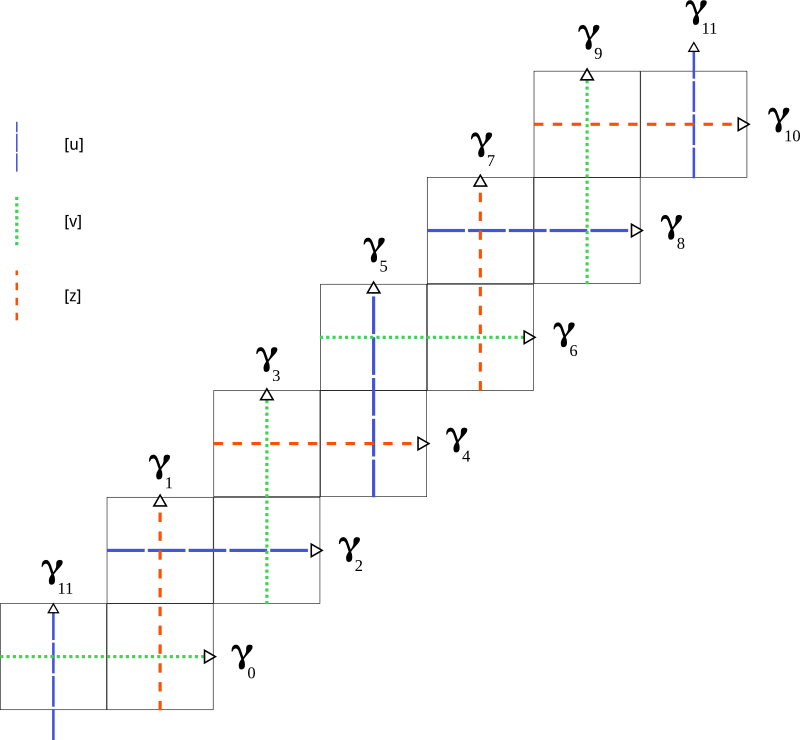
\includegraphics[width=3in]{homologyclass.png}
\centering
\caption{Cylinder core curves with u,v, and z homology classes that determines the $\mathbf{T}^{m,n}$-cover.}
\label{fig:homology}
\end{figure}

\begin{rem}
Although the genus of $\mathbf{M}$ is 5, we use 12 curves as an overdetermined basis for $H_1(\mathbf{M},\mathbb Q)$. To show that they indeed span all of $H_1(\mathbf{M},\mathbb Q)$, it is possible to construct a $12\times12$ matrix of curve intersections and calculate its rank. The rank of the matrix, as to be expected, is 10. But to use only the linearly independent curves means that many of the same symmetries described in the previous section would not induce isomorphisms of $\pi_1(\mathbf{M})$ that dualize $\mathbf{M}$'s symmetries as the union of 12 identical squares.
\end{rem}

We will denote the group of isomorphisms of $\mathbf{M}$'s fundamental group we obtain from $\mathbb{X}$ as $\mathbb X_*$. The same notation will be used for the isomorphisms themselves. We denote the \emph{set of cylinder core curves} as $\Gamma\subset H_1(\mathbf{M},\mathbb Q)$.

\vspace{0.1in}

\noindent\textbf{A 12-gon dualization of the $H_1(\mathbf{M},\mathbb Q)$}

The 12-gon was mentioned in the previous section under the discussion of $\mathbf{M}$'s translational symmetries. $\mathbb X_*$ acting on absolute homology is better represented as this symmetric object.

\begin{figure}[H]
\centering
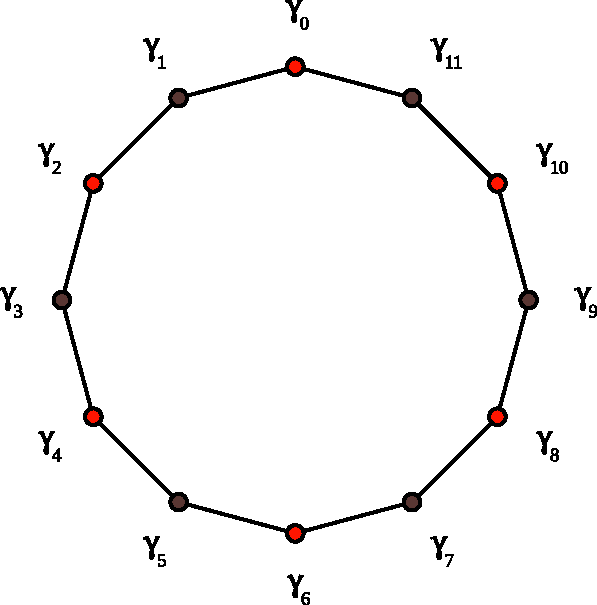
\includegraphics[width=1.7in]{12gon.pdf}
\end{figure}

This graph's representation also reflects how two core curves are incident with only two others. An element of $\mathbb X_*$ either permutes these curves or, in the case where $\mathbf A_*$ or $\mathbf B_*$ generates the element, adds/subtracts black vertices to/from the red ones. Recall that in the previous section we had certain conventions when it came to the elements $\mathbf{R}$, $\mathbf{H}$, and $\mathbf{V}$. This was so that their induced isomorphisms would \emph{fix} one or more vertices as they act on homology. Because of the translational symmetries, it is possible to rotate or reflect entire 12-gon with $\mathbf{H}_*$ and $\mathbf{V}_*$. These permutations of $\Gamma$ generate a group isometric to $\mathbb{D}_{12}$.


\begin{minipage}{0.5\textwidth}
\vspace{0.3in}
\begin{itemize}
\item[\textbf{\emph{$\mathbf{H}_*$\& $\mathbf{V}_*$}}] The effect that these two have on the 12-gon is a reflection about these lines. Observed by keeping track of the squares and core curves after $\mathbf{H}$ and $\mathbf{V}$ have acted on $\mathbf{M}$.
\end{itemize}
\end{minipage}
\begin{minipage}{0.7\textwidth}
\begin{figure}[H]
\hspace{0.2in}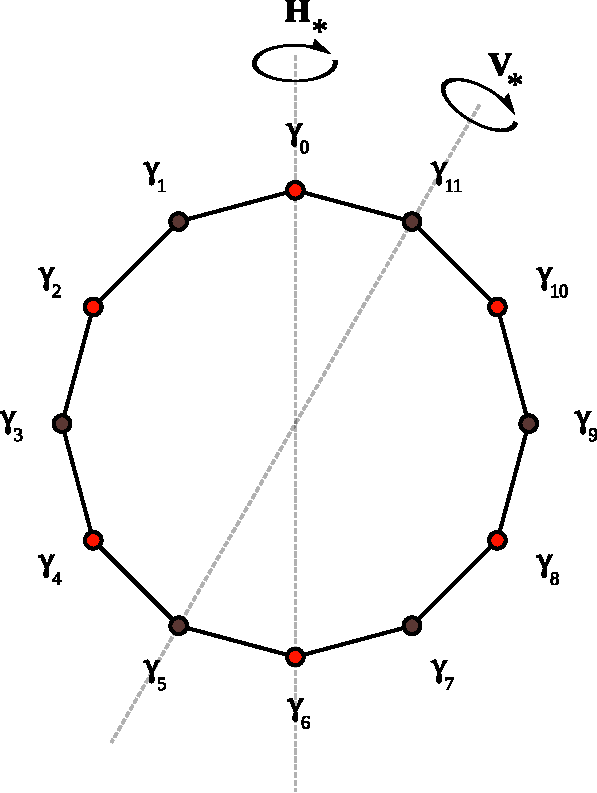
\includegraphics[width=1.7in]{12gonHV.pdf}
\end{figure}
\end{minipage}

The two preserve the signs of the core curves. It is to be expected as they are induced isomorphisms of translations. They are expressed as:
\space
\begin{align*}
\mathbf{H}_* &= (\gamma_0)(\gamma_1\hspace{1mm}\gamma_{11})(\gamma_2\hspace{1mm}\gamma_{10})(\gamma_3\hspace{1mm}\gamma_9)(\gamma_4\hspace{1mm}\gamma_8)(\gamma_5\hspace{1mm}\gamma_7)(\gamma_6)\\
\mathbf{V}_* &=(\gamma_{11})(\gamma_0\hspace{1mm}\gamma_{10})(\gamma_1\hspace{1mm}\gamma_{9})(\gamma_2\hspace{1mm}\gamma_8)(\gamma_3\hspace{1mm}\gamma_7)(\gamma_4\hspace{1mm}\gamma_6)(\gamma_5)
\end{align*}

Rotation about the center of a square will not only change signs of the core curves, but permute elements in such a way that the rotation element is order four.

\begin{minipage}{0.4\textwidth}
\begin{figure}[H]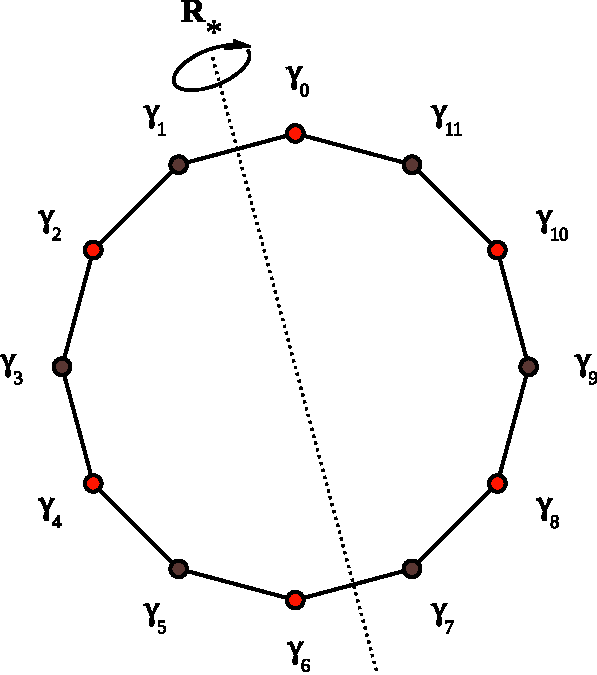
\includegraphics[width=1.7in]{12gonR.pdf}
\end{figure}
\end{minipage}
\begin{minipage}{0.55\textwidth}
\vspace{0in}
\begin{itemize}
\item[\textbf{\emph{$\mathbf{R}_*$}}] This action reflects the 12-gon about that line and maps one vertex to another. No vertex is fixed. However it has the additional effect of changing the sign of a curve only if it was originally black (or odd index).
\end{itemize}
\end{minipage}

\vspace{2mm}
We can see the effect that it has on homology clearer as a permutation group on $\Gamma$:
\begin{align*}
\mathbf{R}_*= \hspace{1mm} &(\gamma_{0}\hspace{1mm}\gamma_{1}\hspace{1mm}\text{-}\gamma_{0}\hspace{1mm}\text{-}\gamma_{1})
(\gamma_{2}\hspace{1mm}\gamma_{11}\hspace{1mm}\text{-}\gamma_{2}\hspace{1mm}\text{-}\gamma_{11})
(\gamma_{3}\hspace{1mm}\text{-}\gamma_{10}\hspace{1mm}\text{-}\gamma_{3}\hspace{1mm}\gamma_{10})\\
&(\gamma_{4}\hspace{1mm}\gamma_{9}\hspace{1mm}\text{-}\gamma_{4}\hspace{1mm}\text{-}\gamma_{9})
(\gamma_{5}\hspace{1mm}\text{-}\gamma_{8}\hspace{1mm}\text{-}\gamma_{5}\hspace{1mm}\gamma_{8})
(\gamma_{6}\hspace{1mm}\gamma_{7}\hspace{1mm}\text{-}\gamma_{6}\hspace{1mm}\text{-}\gamma_{7}).
\end{align*}

\compav{TODO: Make the parabolic 12-gon image.}

\begin{figure}[H]
\centering
\includesvg{12gonA}
\end{figure}

\begin{figure}[H]
\centering
\includesvg{12gonABexample}
\end{figure}
\compav{Ended here August 3.}

\subsection{$\mathbf{T}^{m,n}$-Cover of $\mathbf M$}
When defining $\mathbf{M}$ as a quotient over the action of $\mathbf{T}^{m,n}$, the result was a finite-type translation surface whose cover indexes these four "cut-open tori" by the integer pair $(m,n)$. For this reason it is easy to consider $\tilde{\mathbf{U}}$ to be a kind of $\mathbb{Z}^2$-esque covering space of $\mathbf{M}$.


\begin{lem}
The family of translational symmetries $\mathbf{T}^{m,n}$ is isomorphic to $\mathbb Z^2$.
\begin{proof}
$\mathbf{T}^{m,n}$ is induced by rotational and translational symmetries of the fundamental domain of $\tilde{\mathbf{U}}$, $\mathbf P \times \mathbb{Z}/4\mathbb{Z}$. It's clear that the rotations themselves are bijective maps. By definition, $\mathbf{T}_0^{m,n}=(x+2m,y+2n;j)$. As a group action, observe that the points $(x,y;j)$ are stabilized. The orbit of this triple is the set of infinitely many points in its domain parametrized by integers $m,n$. The obvious isomorphism identifies an element of $\mathbb{Z}^2$ with $(m,n)$. The orbit of any point is itself given as $\mathbf{T}_0^{\mathbb Z^2}$. Therefore, the induced map on $\tilde{\mathbf{U}}$, $\mathbf{T}^{m,n}$, is isomorphic to $\mathbb Z^2$ as well.
\end{proof}
\end{lem}

From figure $\ref{fig:mtilda}$ we construct homology classes $u,v$ according to the outer edges of the tori. In addition, there is a class $z$ that doesn't play a role in determining the cover $\tilde{\mathbf U}$. This is because $z$ is the set of core curves that lie on cylinders that go from one plane to the next. Figure $\ref{fig:homology}$ labels them on the staircase model.

\begin{align*}
u &= -\gamma_2 +\gamma_5 + \gamma_8 - \gamma_{11},\\
v &= +\gamma_0 -\gamma_3 -\gamma_6 +\gamma_9,\\
z &= +\gamma_1 +\gamma_4-\gamma_7-\gamma_{10}.
\end{align*}

Let i be a bilinear, non-degenerate form given as

\begin{align}
i:H_1(\mathbf{M},\mathbb Q)\times H_1(\mathbf{M},\mathbb Q)\rightarrow \mathbb Z.
\end{align}

Let $\beta\in \pi_1(\mathbf{M}, x_0)$, and $[\beta]$ be its abelianization in $H_1(\mathbf{M},\mathbb{Q})$.
The function returns an \emph{intersection number} between two elements in $H_1(\mathbf{M},\mathbb Q)$. Assuming that $[\beta]$ is the second argument of i, a positive crossing occurs when $[\beta]$'s angle of intersection with the first homology class is positive. Fix a point $x_0\in\mathbf{M}$. $x_0$ lifts to $\tilde{x}_0\in\tilde{\mathbf{U}}$ by the covering map $f$, such that $\tilde{x}_0$ belongs to the quotient of $\tilde{\mathbf{U}}$ indexed $\mathbf{T}^{0,0}$.

$\tilde{\mathbf{U}}$ is associated to the kernel of the group homomorphism,
\begin{align}
\Omega_{u,v}:\pi_1(\mathbf{M},x_0)\rightarrow \mathbb{Z}^2 \text{; } \beta\mapsto(i(u,[\beta]),i(v,[\beta])).
\end{align}
Since $\mathbf{T}^{m,n}$ is isomorphic to $\mathbb{Z}^2$, the lift of $\beta\in \text{Ker } \Omega_{u,v}$ is the closed path, $\tilde{\beta}$. Let $F^t_\theta$ be a \emph{non-singular} geodesic flow on $\mathbf{M}\backslash$Sing$(\mathbf M)$ with initial point $x_0$. By [some theorem], $F^t_\theta$ is closed for for every rational direction $\theta$. The image of $F^t_\theta$ is an element of $\pi_1(\mathbf M, x_0)$, and homotopic to closed path $\beta$. 

\begin{Def} Identify $\mathbb C$ with $\mathbb{R}^2$ in the usual way. The closed path $\alpha\in\pi_1(\mathbf M, x_0)$ is the path contained in the maximal cylinder decomposition of $\mathbf M$ in direction $(1,1)$ with hol$(\alpha)=6+6i$.
\end{Def}

\begin{figure}[H]
\centering
\includesvg[pretex=\tiny, width=4.5in]{slopeonecylinder}
\caption{In the slope one direction, $\mathbf M$ decomposes into two cylinders.}
\end{figure}

We can see that $hol(\alpha)=6+6i$ is the holonomy vector of the closed loop $\alpha$ contained in one of these cylinders. Call the unlabeled cylinder $C_1$(right), and the labeled one $C_2$(left).


\begin{lem}
$\alpha$ is homologous to the image of the closed geodesic in direction $(1,1)$ on $\mathbf{M}\backslash\text{Sing}(\mathbf M)$.
\begin{proof}
Let $\chi$ be a separatrix contained in either $C_1$ or $C_2$. Since a separatrix does not admit singularities, it is the image of a closed geodesic on $\mathbf{M}\backslash\text{Sing}(\mathbf M)$ with initial point $x_0$ on the strips of $C_1$ and $C_2$ with boundaries removed, denoted $C_1',$ $C_2'$. Express $[\alpha]$ as $\Sigma^{11}_{j=0}$ $\frac{1}{2}\gamma_j$ (a closed path climbing up the staircase). We show that the intersection numbers of $[\alpha]$ and $[\chi]$ are the same for every core cylinder curve $\gamma$, i.e. $i([\gamma_k], \Sigma^{11}_{j=0} \text{ } \frac{1}{2}[\gamma_j])=i([\gamma_k],[\chi])\text{ } \forall k=0,\dots,11$.    \\
\textbf{Case one:} k is even. If k is even, then every curve $\gamma_k$ is oriented to the right. Since $\chi$ intersects every curve once, $i([\gamma_k],[\chi])=1$. No even indexed curves intersect eachother, so we need only consider when $j$ is odd. Now if $j$ is odd, it is incident (positively crossing) with only two horizontal curves, namely $\gamma_{j+1},\gamma_{j-1}$. Therefore $i([\gamma_k],[\alpha])=i([\gamma_{j-1}],\frac{1}{2}[\gamma_{j}])+i([\gamma_{j+1}],\frac{1}{2}[\gamma_{j}])=\frac{1}{2}(i([\gamma_{j-1}],[\gamma_{j}])+i([\gamma_{j+1}],[\gamma_{j}]))=\frac{1}{2}(1+1)=1.$\\
\textbf{Case two:} k is odd. If k is odd, then $[\chi]$ will have an intersection number of $-1$ with $[\gamma_k]$ since odd-indexed core curves are oriented upwards. Now since k is odd, we only consider when $j$ is even. Similarly, this means that $\gamma_j$ negatively intersects the two vertical core curves with adjacent indices. Hence, $i([\gamma_k],[\alpha])=i([\gamma_{j-1}],\frac{1}{2}[\gamma_{j}])+i([\gamma_{j+1}],\frac{1}{2}[\gamma_{j}])=\frac{1}{2}(i([\gamma_{j-1}],[\gamma_{j}])+i([\gamma_{j+1}],[\gamma_{j}]))=\frac{1}{2}(-1-1)=-1.$\\
We know intersection number to be non-degenerate, and since $\alpha$ and $\chi$'s abelianizations admit the same intersection numbers for every curve in the spanning set of $H_1(\textbf M, \mathbb{Q})$,  $[\alpha]=[\chi]$.
\end{proof}
\end{lem}

We will abuse notation occasionally and refer to $\alpha$ as the geodesic of slope one. In the horizontal direction, (1,0), $\mathbf{M}$ has the 6 cylinder decomposition shown in figure $\ref{fig:decomp}$. A similar argument shows that any horizontal cylinder curve is homotopic to a curve with holonomy vector 2 on the cylinder. The core curves themselves are geodesics on the surface that intersect only two other curves, which is a property used in the previous theorem. Their intersection numbers are therefore zero everywhere except for the curves with adjacent indices. This is unlike $\alpha$, which intersects every curve exactly once. Oftentimes we consider $\alpha$ to travel around the 12-gon counterclockwise, intersecting negatively with odd-indexed $\gamma$ (black nodes), and positively with even-indexed $\gamma$ (red nodes).

The translational and rotational symmetries allows one $\gamma$-curve to end up in the place of any other curve, with positive or negative orientation. For that reason we default to using $\gamma_0$

\begin{rem}
The Infinite Staircase that covers $\mathbf{M}$ has the same shear automorphisms as $\mathbf{M}$, and similar cylinder decompositions as well. In these odd-odd directions, it decomposes into two cylinders of infinite area. In even-odd directions, it will decompose into countably many cylinders of finite area. [cite]
\end{rem}

\begin{thm}
$\alpha\in\pi_1(\mathbf{M}, x_0)$ lifts to a closed path $\tilde{\alpha}\in\pi_1(\tilde{\mathbf{U}},\tilde{x}_0)$.
\end{thm}
\begin{proof}
As a result of the previous theorem, $i([\gamma_i],[\alpha])=1$ when i is even and $i([\gamma_i],[\alpha])=-1$ when i is odd. Therefore $i([u],[\alpha])=-i([\gamma_2],[\alpha] +i([\gamma_5],[\alpha]) + i([\gamma_8],[\alpha]) - i([\gamma_{11}],[\alpha])=-1+(-1)+1-(-1)=0$, and $i([v],[\alpha])=1-(-1)-1+(-1)=0$. So $\Omega_{u,v}(\alpha)=(0,0)\simeq \mathbf{T}^{0,0}$, by Lemma 3.2. As such $\alpha\in$ Ker $\Omega_{u,v}$, and lifts to a closed path on $\tilde{\mathbf{U}}$.
\end{proof}

\begin{thm}
The lift of core curves $\Gamma$ on $\tilde{\mathbf{U}}$ are drift-periodic.
\end{thm}
\begin{proof}
\compav{show that intersection with u,v will only get one of 1, 0, or -1. therefore i(x,y) is never (0,0)}
\end{proof}



\begin{figure}[H]
\centering
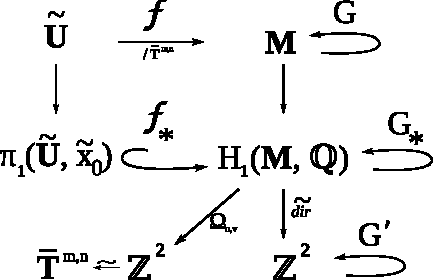
\includegraphics{z2cover.pdf}
\caption{\compav{Fix this!}}
\end{figure}

\begin{conj}{\textbf{Periodicity of Geodesic Flow on the Necker cube surface.}}\\ Let $\theta$ be a direction obtained described as in Definition 3. Denote the geodesic flow on $\mathbf{S}$ by $F^t_{[\theta]}:T^1_{\bar{\Psi}(s)}(\mathbf{U}\backslash Sing(\mathbf U))\times\mathbb{R}_0^+\rightarrow\mathbf{S}$, where $F^t_{[\theta]}=\bar{\Psi}^{-1}(\bar{\Psi}(s)+t[\theta])$ for initial point $s\in\mathbf{S}$. Then the following is true:
\begin{enumerate}[label=(\roman*)]
\item If $\theta$ is rational and identified with an element in $\mathcal{O}$, then $F^t_{[\theta]}$ is periodic.
\item If $\theta$ is rational and identified with an element in $\mathcal{E}$, then $F^t_{[\theta]}$ is drift-periodic.
\end{enumerate}
\end{conj}

\newpage
\begin{lem}
The group $\mathbb{X}'$ acting on $\mathbb{Z}^2$ sends $\mathcal{O}$ to $\mathcal{O}$, and $\mathcal{E}$ to $\mathcal{E}$.
\begin{proof}
Since $\mathbb{X}'$ is generated by the elements $\mathbf{A}'$, $\mathbf{B}'$, and $\mathbf{R}'$, any matrix $G'\in\mathbb{X}'$ is of the form $G' = (\mathbf{A}')^{1_1}\circ(\mathbf{B}')^{1_2}\circ(\mathbf{R}')^{1_3}\circ(\mathbf{A}')^{2_1}\circ\dots(\mathbf{A}')^{n_1}\circ(\mathbf{B}')^{n_2}\circ(\mathbf{R}')^{n_3}$, where $i_k\in\mathbb{Z}$ for $i=1,\dots,n$ and $k=1,2,3.$ Let $x=\left(\begin{matrix}p \\ q  \end{matrix}\right),y\in\mathcal{O}$, and consider the equation $G'x=y$. Observe that $\left(\begin{matrix}1 && 2 \\ 0 && 1\end{matrix}\right)^l x=\left(\begin{matrix}p+2jq \\ q  \end{matrix}\right),$ and $ \left(\begin{matrix}1 && 0 \\ 2 && 1\end{matrix}\right)^m x=\left(\begin{matrix}p \\ q+2mp  \end{matrix}\right)$ for any $l,m\in\mathbb{Z}$. Also note that for any $j\in\mathbb{Z}$, $(\mathbf{R}')^{m}x=\left(\begin{matrix}p \\ q  \end{matrix}\right),\left(\begin{matrix}-q\\ p  \end{matrix}\right),\left(\begin{matrix}-p \\ -q  \end{matrix}\right),\left(\begin{matrix}q \\ -p  \end{matrix}\right)$ when $j \mod{4}\equiv0,1,2,3$, respectively. In any case, the product of any power of a generator of $\mathbb{X}'$ and any $x\in\mathcal{O}$ is an element of $\mathcal{O}$ . By letting $l=i_1,m=i_2,$ and $j=i_3$, we first consider the base case when $i=n$. Let $G'=G'_1\circ\dots\circ G'_n$, such that $G'_i=(\mathbf{A}')^{i_1}\circ(\mathbf{B}')^{i_2}\circ(\mathbf{R}')^{i_3}$. Since $n_1,n_2,n_3$ are arbitrary integers, $G'_n x \in\mathcal{O}$. Suppose for some $b< n-1$, $G'_{n-b}\circ\dots\circ G'_n x =y'\in\mathcal{O}$. Therefore $y'=(G'_1\circ\dots\circ G'_{b})^{-1}y$, which implies that $(G'_1\circ\dots\circ G'_{b})^{-1}$ preserves the set $\mathcal{O}$. Otherwise, if $y\in\mathcal{E}$, there exists at least one $G'_i$ for $1< i< b$ and $\tau\in\mathcal{E}$ such that $G'^{-1}_i \tau = (\mathbf{R}')^{-i_3}\circ(\mathbf{B}')^{-i_2}\circ(\mathbf{A}')^{-i_1} \tau \in \mathcal{O}$, a contradiction. Since elements in $\mathbb{X}'$ are invertible, $G'_1\circ\dots\circ G'_{b}$ must also preserve $\mathcal{O}$. By inductive reasoning, we conclude that  $G'_1\circ\dots\circ G'_n x = G' x = y$. $x\in\mathcal{O}$ if and only if $y\in\mathcal{O}$ since $G'$ is invertible.\\
Proving that $G'(\mathcal{E})=\mathcal{E}$ is done in the same way.
\end{proof}
\end{lem}


\end{document}
